\documentclass[11pt]{article}
\usepackage[margin=1in]{geometry}
\usepackage{amsmath,amssymb,amsthm,mathtools}
\usepackage{enumitem}
\usepackage{xcolor}
\usepackage{graphicx}
\usepackage{float}
\graphicspath{{../../results/}}
\usepackage[colorlinks=true,linkcolor=blue!50!black,citecolor=blue!50!black,urlcolor=blue!50!black]{hyperref}

\newtheorem{theorem}{Theorem}
\newtheorem{lemma}[theorem]{Lemma}
\newtheorem{proposition}[theorem]{Proposition}
\newtheorem{corollary}[theorem]{Corollary}
\theoremstyle{definition}
\newtheorem{assumption}{Assumption}
\newtheorem{remark}[theorem]{Remark}
\newtheorem{conjecture}[theorem]{Conjecture}

\newcommand{\E}{\mathbb{E}}
\newcommand{\R}{\mathbb{R}}
\newcommand{\Nb}{N_{\mathrm b}}
\newcommand{\Xmax}{X_{\max}}
\newcommand{\eps}{\varepsilon}
\DeclareMathOperator*{\argmax}{arg\,max}

\title{Fed-ZoomSIB with a server: what is (and is not) new\\[2pt]
\large Proofs for claims 1.2, 1.3 and 2.1 of \texttt{docs/claims-evidence.md}}
\author{CS6007 project notes}
\date{October 2026}

\begin{document}
\maketitle

\begin{abstract}
We make precise the statement ``with a server, $N$ agents for $T$ rounds are a single agent for
$NT$ rounds''. Theorem~\ref{thm:lower} shows that no $N$-agent algorithm, whatever it
communicates, can beat the single-agent minimax rate at horizon $NT$. Theorem~\ref{thm:upper}
shows that Fed-ZoomSIB with exact sufficient-statistic pooling and event-triggered sync
\emph{attains} that rate. Theorem~\ref{thm:comm} bounds its communication by
$O(\Nb\log_{1+\gamma}(NT))$ sync rounds, and Proposition~\ref{prop:share} shows that Phase~1 is an
$O(d/(NT)^{1/3})$ fraction of all traffic. Section~\ref{sec:dec} sketches the serverless
(relay) version, whose bound carries an additive $O(N D \Nb)$ term, and
Section~\ref{sec:tradeoff} states the open regret--communication question these results leave.
Imported results from Dey, Bhore \& Ghosh (2026), hereafter \emph{DBG}, are marked as such.
\end{abstract}

\section{Setting}

$N$ agents, $T$ rounds. At round $t$ agent $i$ observes $K$ contexts $x_{i,t,1},\dots,x_{i,t,K}$
drawn i.i.d.\ from $\mathcal D$ on $\R^d$, independently across agents and rounds, pulls
$a_{i,t}$ and observes $y_{i,t}=f(\langle x_{i,t,a_{i,t}},\theta^*\rangle)+\eta_{i,t}$. Both
$\theta^*$ (with $\|\theta^*\|_1=1$) and $f$ are unknown and shared by all agents. Network regret is
\[
R_T(N)=\sum_{i=1}^N\sum_{t=1}^T\Big[\max_{a} f(\langle x_{i,t,a},\theta^*\rangle)-f(\langle x_{i,t,a_{i,t}},\theta^*\rangle)\Big].
\]

\begin{assumption}[DBG Assumptions 1--3]\label{ass}
(i) $\eta_{i,t}$ is independent of the contexts and conditionally $\sigma$-sub-Gaussian given the
past. (ii) $\E[S_j(X)^2]\le M$ for the score $S=-\nabla\log p$. (iii) Each coordinate of $X$ is
$\kappa$-sub-Gaussian; $|f|\le L_f$ and $|f'|\le L_{f'}$ on $|z|\le\Xmax$, where
$\Xmax=\kappa\sqrt{2\log(2dNTK/\delta)}$ bounds $\|x\|_\infty$ for all $NTK$ contexts with
probability $\ge1-\delta$. (iv) $\mu^*=\E[f'(\langle X,\theta^*\rangle)]>0$.
\end{assumption}

\begin{lemma}[Imported: DBG Lemma B.1 with Lemma 2.1]\label{lem:stein}
Let $\hat\theta$ be the truncated Stein estimator $\frac1n\sum_{s=1}^n\varphi_\tau(y_sS(x_s))$
on $n$ i.i.d.\ pairs with $\tau=\sqrt{3(\sigma^2+L_f^2)Mn/\log(2d/\delta)}$, and
$\hat\theta_0=\hat\theta/\|\hat\theta\|_1$. If $n$ is large enough that
$C_\theta d\sqrt{\log(2d/\delta)/n}\le\mu^*/2$, then with probability $\ge1-\delta$
\[
\|\hat\theta_0-\theta^*\|_1\le\eps_0(n):=\frac{4C_\theta d}{\mu^*}\sqrt{\frac{\log(2d/\delta)}{n}},
\qquad C_\theta=\tfrac{4\sqrt3}{3}+2\sqrt2\sqrt{M(\sigma^2+L_f^2)}.
\]
\end{lemma}

\begin{lemma}[Imported: DBG Theorem 5.1]\label{lem:dbglower}
There are $c>0$ and $n_0$ such that for every horizon $n\ge n_0$ and every single-agent policy
$\pi$, $\sup\E[R_n(\pi)]\ge c\,n^{2/3}$, the supremum over instances satisfying the regularity
assumptions (with $d=1$, Gaussian contexts and $K=\lceil 4N'\log n/p_{\min}\rceil$ arms for an
$N'$-bin construction).
\end{lemma}

\section{Lower bound: a network is never better than one agent with all the data}

\begin{theorem}[Lower bound by simulation]\label{thm:lower}
Let $\mathcal A$ be any $N$-agent algorithm, with arbitrary communication, including every agent
seeing every other agent's data after every round. Then for $NT\ge n_0$,
\[
\sup_{\text{instances}}\E[R_T(N;\mathcal A)]\ \ge\ c\,(NT)^{2/3}.
\]
The same holds for every serverless algorithm, since it is a special case.
\end{theorem}

\begin{proof}
We build a single-agent policy $\pi$ with horizon $n=NT$ whose regret has exactly the law of
$\mathcal A$'s network regret; Lemma~\ref{lem:dbglower} then applies to $\pi$.

Index the single agent's rounds by $u=(t-1)N+i$, so that round $u$ plays the role of
``agent $i$ at round $t$''. Policy $\pi$ keeps a copy of $\mathcal A$'s full internal state
(all agents, the server, and their random seeds, which $\pi$ draws itself). At round $u=(t,i)$:
\begin{enumerate}[nosep]
\item $\pi$ observes its context set $X_u$ and passes it to the simulated agent $i$, which
selects $a_u$ using its state \emph{as of the end of round $t-1$}, exactly as in $\mathcal A$.
\item $\pi$ plays $a_u$ and receives $y_u$, but \emph{withholds} it from the simulation.
\item When $i=N$, all $N$ outcomes of round $t$ are available. $\pi$ feeds them to the simulated
agents' updates and runs one round of $\mathcal A$'s communication.
\end{enumerate}
This is a valid policy: each decision uses only information from strictly earlier rounds of
$\pi$.

The context sets $X_u$ are i.i.d.\ from $\mathcal D^K$, and the noise is independent of
everything before it, in both systems. So by induction over $t$, the joint law of
(contexts, actions, rewards) of round $t$ is the same under $\pi$ and under $\mathcal A$, given
the same law up to round $t-1$. In particular $R_{NT}(\pi)\overset{d}{=}R_T(N;\mathcal A)$ on every
instance. Hence
$\sup\E R_T(N;\mathcal A)=\sup\E R_{NT}(\pi)\ge c(NT)^{2/3}$.
\end{proof}

\begin{remark}
The argument uses only that agents are statistically identical (shared $\theta^*,f,\mathcal D$)
and act in parallel. It fails under concept shift (different $\theta^*_i$), which is where
collaboration stops being ``one agent with more data''.
\end{remark}

\section{Upper bound: Fed-ZoomSIB-SS attains the single-agent rate at $NT$}

\paragraph{Algorithm (as analysed).}
\begin{itemize}[nosep]
\item \emph{Phase 1} (rounds $1..T_0$): every agent pulls uniformly at random and stores
$(S(x),y)$. At round $T_0$ each agent uploads $b_i=\sum_{t\le T_0}\varphi_\tau(y_{i,t}S(x_{i,t}))$
and $n_i=T_0$, with $\tau$ set for the pooled size $n=NT_0$. The server broadcasts
$\hat\theta_0=\sum_ib_i/\|\sum_ib_i\|_1$. (Code: \texttt{phase1="exact"},
\texttt{freeze="fixed"}.)
\item \emph{Grid}: window $W=\Xmax$; bins $I_j=(-W+(j-1)\Delta,\,-W+j\Delta]$ for
$j\le\Nb=\lceil2W/\Delta\rceil$. An arm $x$ belongs to bin $b(x)\ni\langle x,\hat\theta_0\rangle$.
\item \emph{Phase 2}: the server holds the synced table $(G_j,G^S_j)$. Agent $i$ holds unsynced
deltas $(\delta n_{i,j},\delta S_{i,j})$ and acts on $n_{i,j}=G_j+\delta n_{i,j}$,
$S_{i,j}=G^S_j+\delta S_{i,j}$. Among the bins its arms fall into, it picks
$\argmax_j\,S_{i,j}/n_{i,j}+w(n_{i,j})$ (with $w(0)=\infty$) and any arm in that bin.
\item \emph{Trigger}: at the end of a round, if some agent has
$\delta n_{l,j}>\gamma\max(G_j,1)$, all agents upload their deltas and the server merges and
broadcasts them. (Code: \texttt{phase2="event"}.)
\end{itemize}
The confidence width is $w(n)=c_\delta\sqrt{2/n}$ with
$c_\delta=\sigma\sqrt{2\log(4N\Nb(NT)^3/\delta)}$. (The code uses the smaller
$\sigma\sqrt{2\log(2\Nb NT/\delta)}$; the difference is a constant and a log factor.)

\begin{lemma}[Phase 1 is exactly centralised]\label{lem:exact}
$\sum_ib_i/(NT_0)$ is the truncated Stein estimator on the pooled $n=NT_0$ samples. These are
i.i.d.\ with the law of single-agent Phase-1 samples. Hence, on an event $E_\theta$ of
probability $\ge1-\delta$, $\|\hat\theta_0-\theta^*\|_1\le\eps_0(NT_0)$.
\end{lemma}
\begin{proof}
Truncation is applied per summand with the same $\tau$, so the sum of agents' sums is the sum
over the pooled sample. Uniform pulls make each $(x,y)$ an independent draw of the context
distribution and the reward model. Apply Lemma~\ref{lem:stein}.
\end{proof}

\paragraph{Good events.}
$E_x$: $\|x\|_\infty\le\Xmax$ for all contexts. $E_\theta$: as in Lemma~\ref{lem:exact}.
$E_\eta$: the noise concentration defined in Lemma~\ref{lem:conf}. On $E_x\cap E_\theta$,
\begin{equation}\label{eq:proj}
|\langle x,\hat\theta_0\rangle-\langle x,\theta^*\rangle|\le\|x\|_\infty\|\hat\theta_0-\theta^*\|_1\le\Xmax\eps_0=:\eps_{\rm p},
\end{equation}
and every arm lies in the window, since $|\langle x,\hat\theta_0\rangle|\le\|x\|_\infty\|\hat\theta_0\|_1\le W$.
Let $\tilde I_j=I_j+[-\eps_{\rm p},\eps_{\rm p}]$ and $m_j=\sup_{z\in\tilde I_j}f(z)$. By
\eqref{eq:proj} every pull into bin $j$ has true index in $\tilde I_j$, so its mean
$\mu_s=f(z_s)$ lies in $[m_j-\omega,m_j]$, where $\omega=L_{f'}(\Delta+2\eps_{\rm p})$.

\begin{lemma}[Confidence for stale, agent-specific tables]\label{lem:conf}
Order all Phase-2 pulls into bin $j$ lexicographically by (round, agent). With probability
$\ge1-\delta$ (event $E_\eta$), for every agent $i$, bin $j$ and round $t$,
\[
\Big|\tfrac{S_{i,j}}{n_{i,j}}-\tfrac1{n_{i,j}}\textstyle\sum_{s\in\text{seen}}\mu_s\Big|\le w(n_{i,j}).
\]
\end{lemma}
\begin{proof}
The pulls agent $i$ sees in bin $j$ are a \emph{prefix} of bin $j$'s sequence (everything up to
the last sync) together with a \emph{contiguous segment} of agent $i$'s own bin-$j$ pulls (since
that sync). The noise along the lexicographic order is a martingale difference sequence: the
bin chosen at $(t,i)$ depends only on rewards of earlier rounds. Azuma--Hoeffding with a union
bound over all prefixes ($\le NT$ per bin) and all segments ($\le(NT)^2$ per agent and bin)
bounds each part's noise sum by $c_\delta\sqrt{\text{length}}$. Then
$\sqrt{p}+\sqrt{q}\le\sqrt{2(p+q)}$ completes the proof.
\end{proof}

\begin{lemma}[Per-pull regret]\label{lem:perpull}
On $E=E_x\cap E_\theta\cap E_\eta$, if agent $i$ pulls from bin $J$ at round $t$, its instant
regret is at most $\min\{2L_f,\ 2w(n_{i,J})+2\omega\}$. This holds for \emph{any} availability
pattern.
\end{lemma}
\begin{proof}
The best arm $x^*$ lies in an available bin $j^*$ with $f(\langle x^*,\theta^*\rangle)\le m_{j^*}$.
By Lemma~\ref{lem:conf},
\[
\mathrm{UCB}_{j^*}\ge(m_{j^*}-\omega)-w+w=m_{j^*}-\omega,
\]
or $\mathrm{UCB}_{j^*}=\infty$. Also $\mathrm{UCB}_J\le m_J+2w(n_{i,J})$. The pulled arm has
mean $\ge m_J-\omega$. Combining with $\mathrm{UCB}_J\ge\mathrm{UCB}_{j^*}$ gives regret
\[
\le(\mathrm{UCB}_J+\omega)-(m_J-\omega)\le2w(n_{i,J})+2\omega.
\]
Rewards are in $[-L_f,L_f]$, which gives the other bound.
\end{proof}

\begin{lemma}[Stale counts]\label{lem:stale}
If a pull is the $k$-th pull into bin $J$ (lexicographic order), then the count its agent acts
on satisfies $n_{i,J}\ge(k-c_N)/(1+N\gamma)$, where $c_N=N(1+\gamma)$.
\end{lemma}
\begin{proof}
The $k-1$ earlier pulls are of three kinds:
\begin{itemize}[nosep]
\item synced, $G_J$;
\item agent $i$'s own unsynced pulls;
\item other agents' pulls agent $i$ has not seen.
\end{itemize}
The last kind are either unsynced, at most $(N-1)\gamma\max(G_J,1)$ because no trigger fired at
the end of round $t-1$, or from round $t$ itself, at most $N-1$. Since $n_{i,J}\ge G_J$:
\begin{itemize}[nosep]
\item if $G_J\ge1$, then $k-1\le n_{i,J}(1+N\gamma)+N$;
\item if $G_J=0$, then $n_{i,J}\ge k-1-(N-1)(1+\gamma)$.
\end{itemize}
Both cases imply the claim.
\end{proof}

\begin{theorem}[Upper bound]\label{thm:upper}
Under Assumption~\ref{ass}, with $\delta=1/(NT)$, $\Delta=(NT)^{-1/3}$, $\gamma=\gamma_0/N$, and
$NT_0=\big\lceil(L_{f'}\Xmax\tfrac{4C_\theta d}{\mu^*}\sqrt{\log(2dNT)}\,NT/L_f)^{2/3}\big\rceil$
(and at least the size Lemma~\ref{lem:stein} requires),
\begin{align*}
\E R_T(N)\le{}&
\underbrace{2L_f NT_0}_{\text{Phase 1}}
+\underbrace{4\sqrt2\,c_\delta\sqrt{(1+\gamma_0)\Nb NT}}_{\text{UCB}}
+\underbrace{2L_{f'}\Delta NT}_{\text{discretisation}}\\
&+\underbrace{4L_{f'}\Xmax\eps_0(NT_0)NT}_{\text{projection}}
+\underbrace{2L_f\Nb(c_N+1)}_{\text{staleness}}
+6L_f,
\end{align*}
which is $\tilde O\big((d\,NT)^{2/3}+N(NT)^{1/3}\big)=\tilde O\big(d^{2/3}(NT)^{2/3}\big)$ for
$N\le\sqrt T$. This matches Theorem~\ref{thm:lower} in $N$ and $T$ up to logarithms: the server
setting is ``one agent with $NT$ pulls'', and no faster.
\end{theorem}
\begin{proof}
Phase-1 pulls cost at most $2L_f$ each. On the failure event (probability $\le3\delta$) regret is
at most $2L_fNT$, giving the $6L_f$ term. On $E$, sum Lemma~\ref{lem:perpull} over the pulls into
bin $j$, using Lemma~\ref{lem:stale} for the $k$-th pull:
\begin{align*}
\sum_{k=1}^{n_j}\min\Big\{2L_f,\ 2c_\delta\sqrt{\tfrac{2(1+N\gamma)}{k-c_N}}+2\omega\Big\}
&\le 2L_f(c_N+1)+4\sqrt2\,c_\delta\sqrt{(1+N\gamma)n_j}+2\omega n_j.
\end{align*}
Summing over bins, Cauchy--Schwarz gives $\sum_j\sqrt{n_j}\le\sqrt{\Nb NT}$. Expanding $\omega$
gives the discretisation and projection terms. With $\Delta=(NT)^{-1/3}$ we have
$\Nb\le2\Xmax(NT)^{1/3}+1$, so the UCB and discretisation terms are $\tilde O((NT)^{2/3})$. The
choice of $NT_0$ balances $2L_fNT_0$ against the projection term
$\propto d\,NT/\sqrt{NT_0}$; both become $\tilde O((dNT)^{2/3})$. Finally,
$2L_f\Nb c_N=\tilde O(N(NT)^{1/3})\le\tilde O((NT)^{2/3})$ when $N\le\sqrt T$.
\end{proof}

\begin{remark}[On the $d$-dependence]
DBG state $\tilde O(d^2T^{2/3})$ for one agent. The cruder per-pull argument above
(Lemma~\ref{lem:perpull}, projection error charged to every pull) gives a leading term
$(dNT)^{2/3}$, plus a lower-order $d^2/\mu^{*2}$ burn-in from Lemma~\ref{lem:stein}'s sample-size
condition. This difference in $d$ has not been cross-checked against DBG's proof and should be
verified before it is claimed. The $N$ and $T$ dependence, which is what claim 1.2 concerns, does
not rely on it.
\end{remark}

\begin{remark}[Constant $\gamma$]
The code and experiments use a constant $\gamma=0.5$. Then $\sqrt{1+N\gamma}$ inflates the UCB
term by up to $\sqrt N$ in the \emph{bound}. E22 finds no such loss in practice: the
event-triggered run matches per-round sync.
\end{remark}

\begin{figure}[H]
\centering
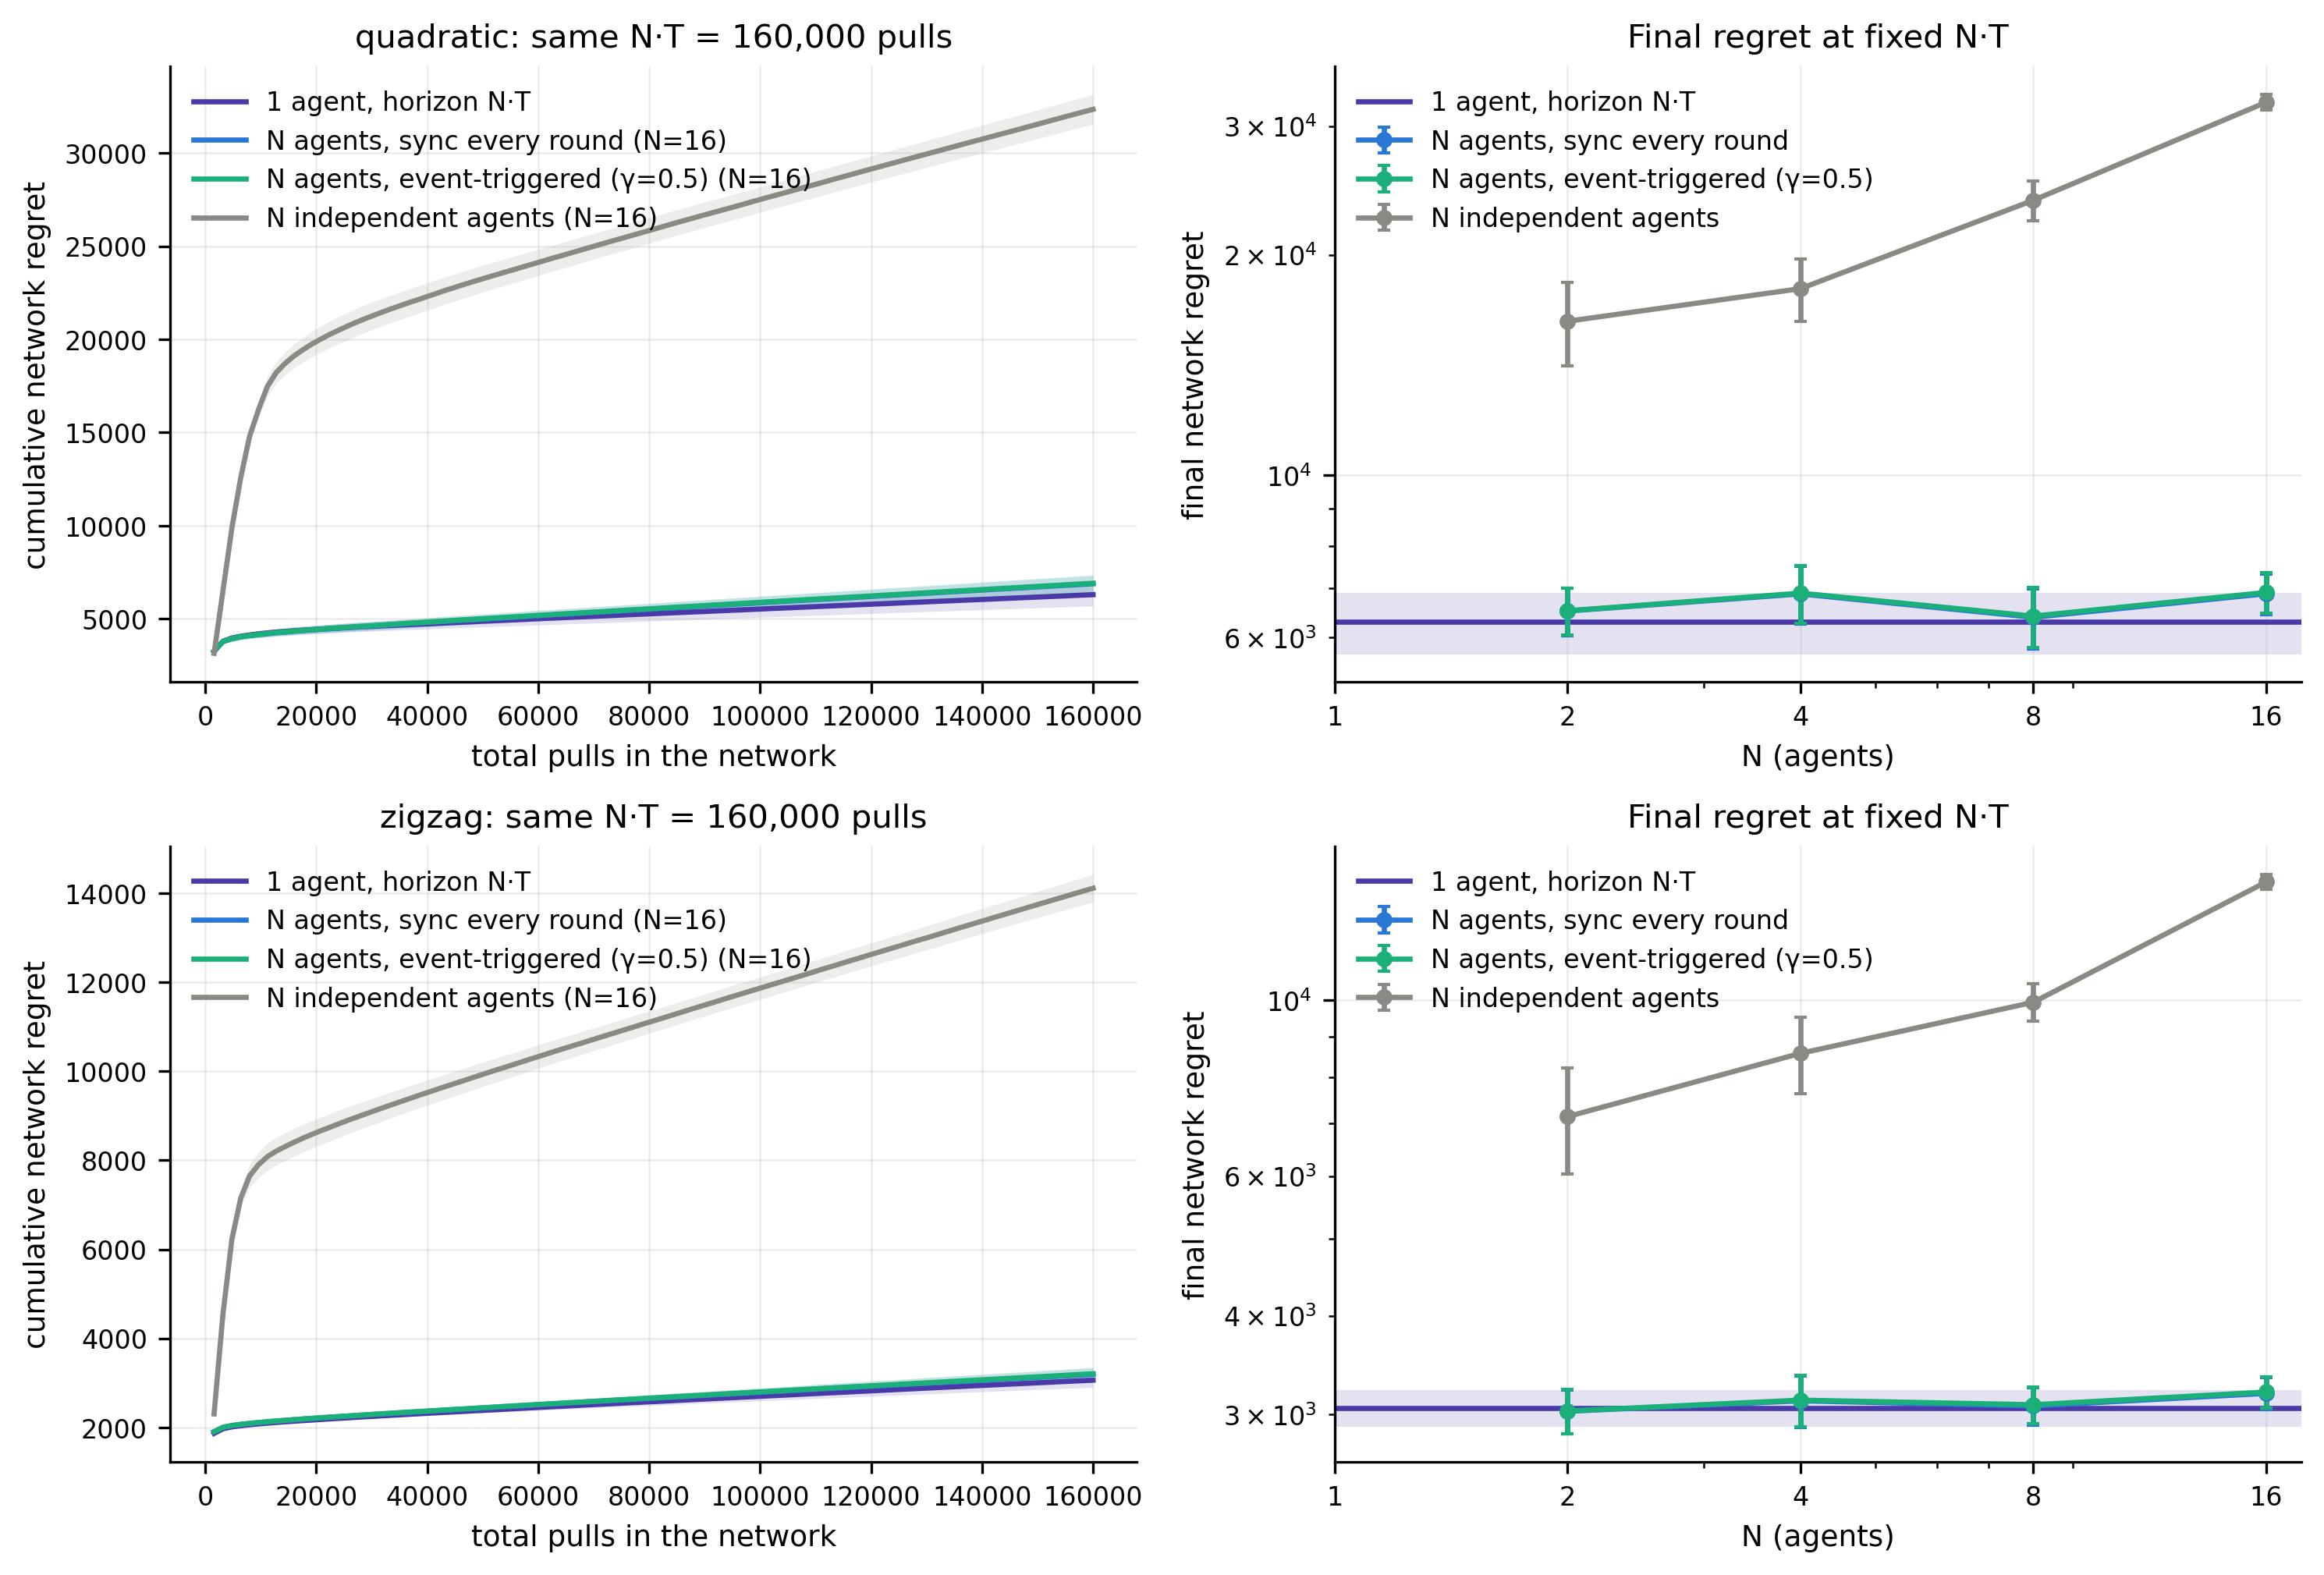
\includegraphics[width=0.92\textwidth]{fig22_single_vs_network.png}
\caption{Empirical check of Theorems~\ref{thm:lower} and~\ref{thm:upper} (E22, 20 paired trials). Fixed total budget $NT=160\,000$, same pooled exploration and bin width for every $N$. Left: regret against total pulls; the single agent at horizon $NT$ and $N=16$ synced agents overlap. Right: final regret against $N$; synced agents stay within 0--10\% of the single agent and never beat it, while independent agents are 2.3--5.1$\times$ worse.}
\label{fig:e22}
\end{figure}

\section{Communication}

\begin{theorem}[Sync rounds]\label{thm:comm}
Phase~2 of Fed-ZoomSIB-SS performs at most
\[
\sum_{j\ \text{used}}\big(1+\log_{1+\gamma}n_j\big)\ \le\ \Nb\Big(1+\log_{1+\gamma}\tfrac{NT}{\Nb}\Big)
\]
sync rounds, where $n_j$ is the final number of pulls in bin $j$. Per-round sync uses $T-T_0$.
\end{theorem}
\begin{proof}
Charge each sync to one bin $j$ whose trigger fired, i.e.\ $\delta n_{l,j}>\gamma\max(G_j,1)$ for
some $l$. The sync adds at least $\delta n_{l,j}$ to $G_j$:
\begin{itemize}[nosep]
\item if $G_j=0$, it becomes $\ge1$;
\item otherwise $G_j$ grows by a factor of at least $1+\gamma$.
\end{itemize}
Since $G_j\le n_j$, bin $j$ is charged at most $1+\log_{1+\gamma}n_j$ times. Bins never pulled are
never charged. Concavity of $\log$ and $\sum_jn_j\le NT$ give the second form.
\end{proof}

\begin{corollary}[Scalars]
Each sync sends 3 scalars per (agent, touched bin) up and 3 per merged bin to each of $N$ agents
down. Every pull is uploaded once, so uploads total at most $3NT$. Downloads total at most
$3N\Nb$ per sync, so at most $3N\Nb^2(1+\log_{1+\gamma}NT)$ overall, which is $\tilde
O(N(NT)^{2/3})$ for $\Delta=(NT)^{-1/3}$. Per-round sync downloads up to
$3N\min(N,\Nb)(T-T_0)$.
\end{corollary}

\begin{remark}[The bound is loose in practice]
E22 measures 61--213 sync rounds for $NT=10^4$--$3.2\cdot10^5$ ($N=8$), against a bound of
3\,600--15\,600, i.e.\ 60--75$\times$ lower. The busiest bin triggers about 3 syncs, against
$1+\log_{1+\gamma}(NT)\approx24$--$32$.
The worst case of Theorem~\ref{thm:comm} assumes every bin is pulled heavily. Sleeping UCB
concentrates pulls on a few near-optimal bins, and most bins trigger at most once. A
gap-dependent communication bound is open (Section~\ref{sec:tradeoff}).
\end{remark}

\begin{figure}[H]
\centering
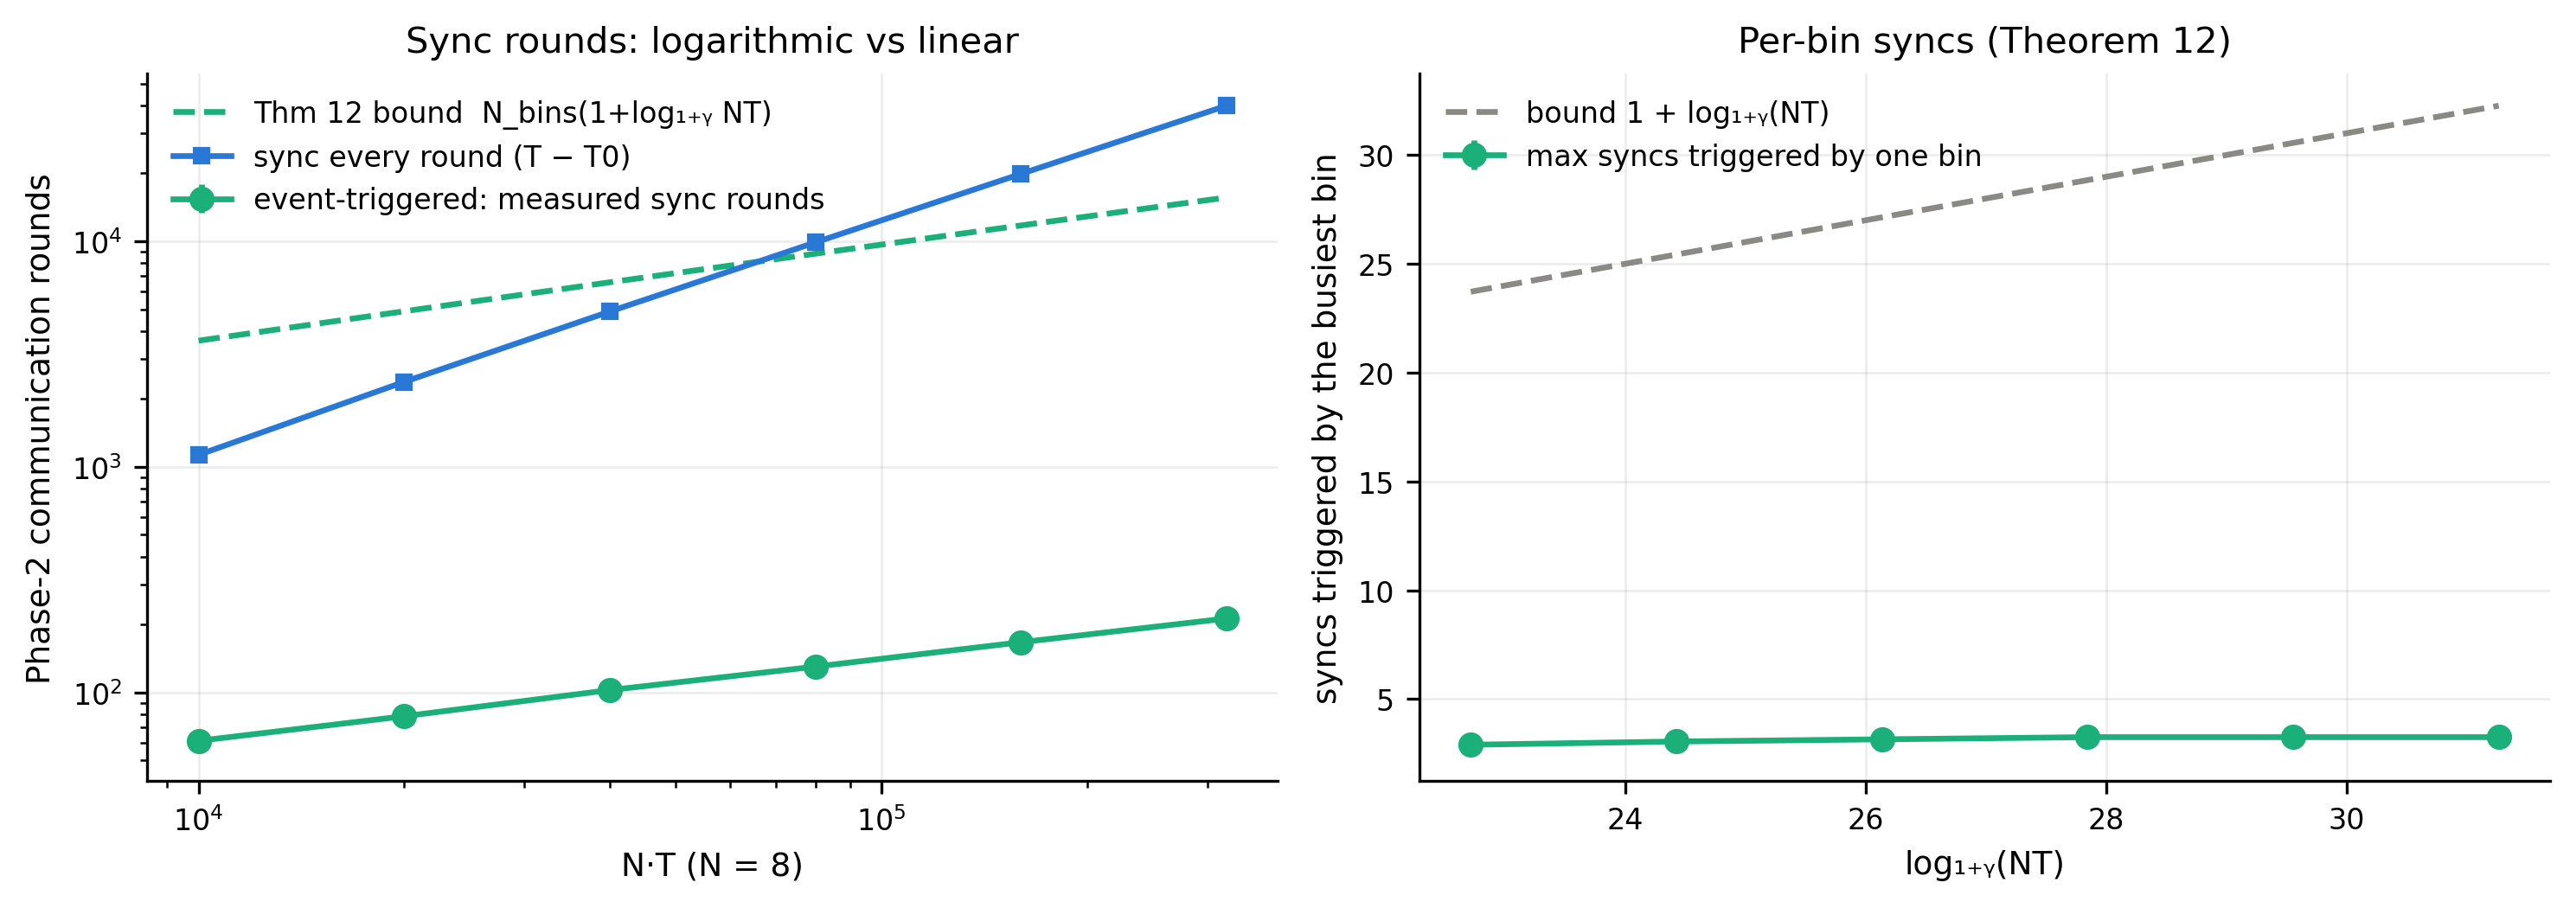
\includegraphics[width=\textwidth]{fig22b_sync_rounds.png}
\caption{Empirical check of Theorem~\ref{thm:comm} (E22 part 2, $N=8$). Left: Phase-2 sync rounds of the event trigger grow logarithmically (61$\to$213 as $NT$ grows 32$\times$) while per-round sync grows linearly; the theorem's bound (dashed) is 60--75$\times$ above the measurement. Right: the busiest bin triggers about 3 syncs against a per-bin bound of 24--32.}
\label{fig:e22b}
\end{figure}

\begin{proposition}[Phase 1 is a vanishing share]\label{prop:share}
With fixed $T_0$, Phase~1 sends $N(2d+3)$ scalars: one $(d+1)$-vector up per agent, $\max|z|$ up,
and $(\hat\theta_0,W)$ down. Suppose $\gamma<1$, and let $\Nb^{\rm used}$ be the number of bins
ever pulled in Phase~2. Then Phase~2 sends at least $3N\Nb^{\rm used}$ scalars, so
\[
\frac{\text{Phase-1 scalars}}{\text{all scalars}}\ \le\ \frac{2d+3}{2d+3+3\Nb^{\rm used}}.
\]
\end{proposition}
\begin{proof}
With $\gamma<1$, a first pull into an empty bin makes $\delta n=1>\gamma\max(0,1)$, so the bin is
merged at the next sync and broadcast (3 scalars) to all $N$ agents at least once.
\end{proof}

\noindent Since $\Nb^{\rm used}$ grows like $(NT)^{1/3}$ until most of the window is visited, the
share is $O(d/(NT)^{1/3})$. Phase~1 matters only when $d$ is comparable with $(NT)^{1/3}$. E24
measures under 2\% at $d\le100$, and compressing Phase~1 saves at most that share.

\begin{figure}[H]
\centering
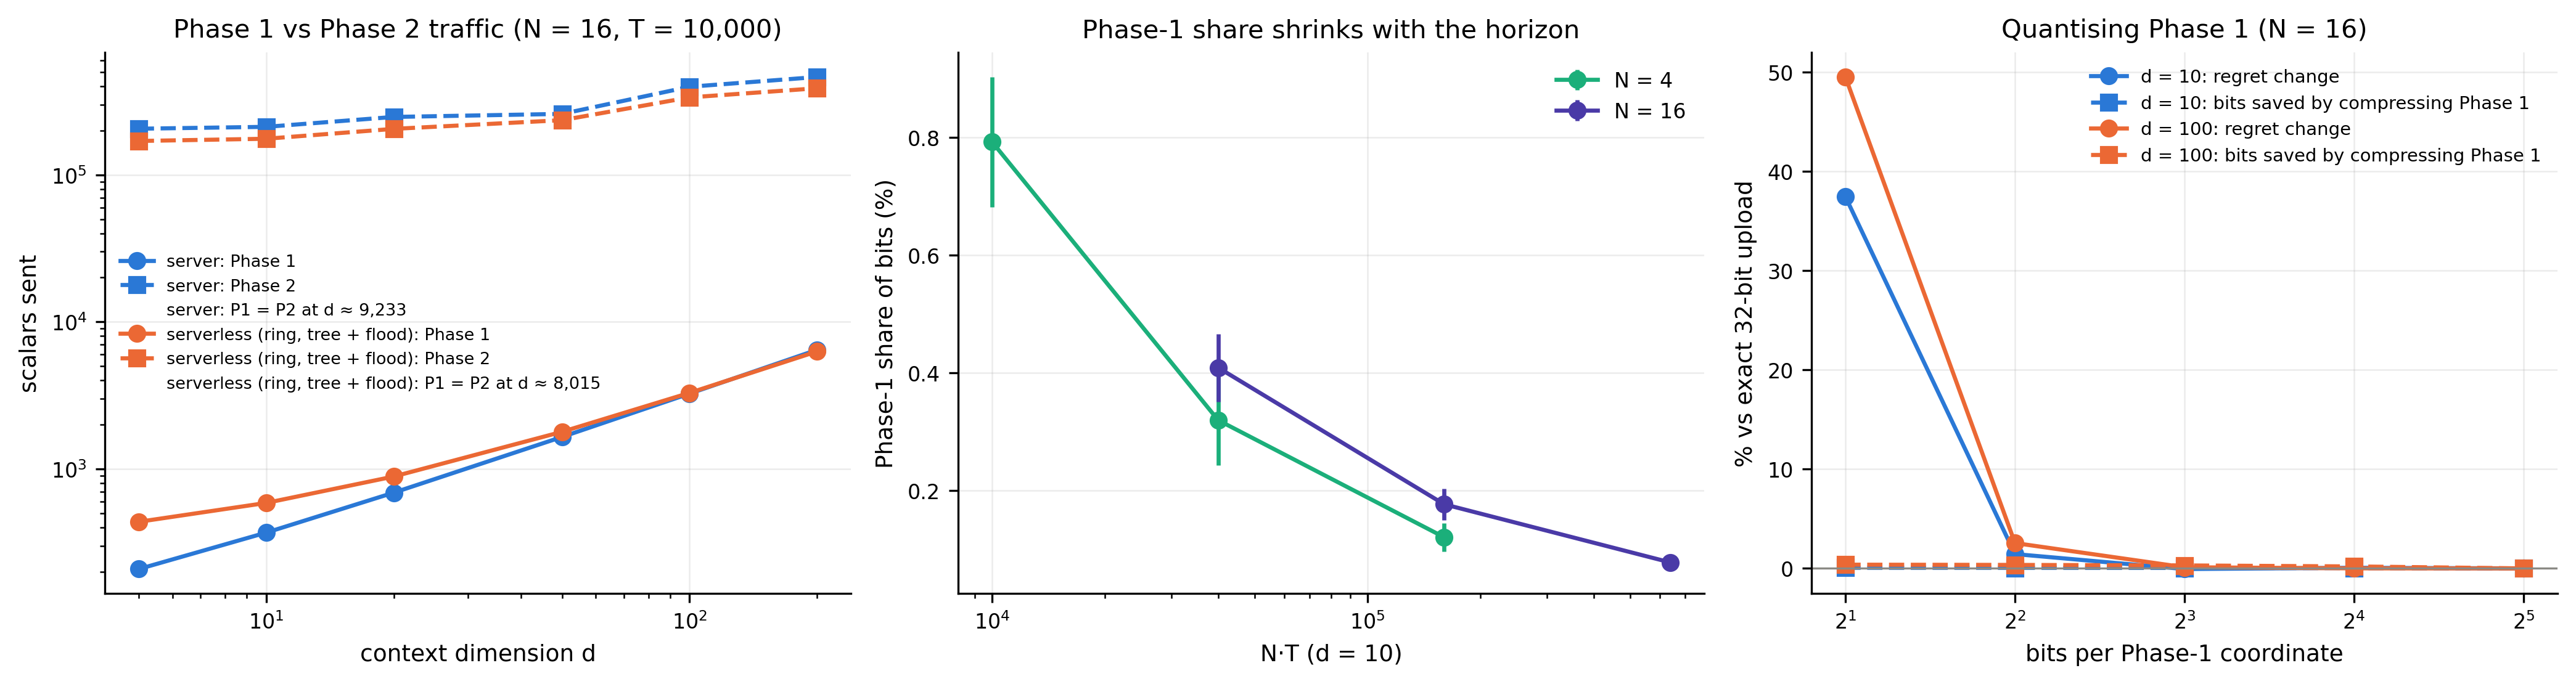
\includegraphics[width=\textwidth]{fig24_phase1_share.png}
\caption{Empirical check of Proposition~\ref{prop:share} (E24). Left: Phase-1 traffic grows linearly in $d$, Phase-2 traffic is far larger for every $d\le200$, server and serverless. Middle: the Phase-1 share falls as $NT$ grows, as $O(d/(NT)^{1/3})$ predicts. Right: quantising the Phase-1 upload saves at most 0.06--0.38\% of all bits, while 2-bit rounding costs 37--50\% regret.}
\label{fig:e24}
\end{figure}


\section{Without a server: the relay version (sketch)}\label{sec:dec}

Dec-ZoomSIB-Relay replaces the server as follows:
\begin{itemize}[nosep]
\item spanning-tree aggregation in Phase~1, which is exact, so Lemma~\ref{lem:exact} holds after
$2\cdot$depth extra exploration rounds;
\item event-triggered \emph{flooding} of each agent's own bin table in Phase~2: records travel one
hop per round, and agent $l$ republishes when its unpublished count exceeds $\gamma$ times its
current view.
\end{itemize}

\begin{theorem}[Relay, sketch]\label{thm:relay}
On a connected graph of diameter $D$, with the parameters of Theorem~\ref{thm:upper}, the relay
version satisfies $\E R_T(N)\le(\text{bound of Thm.~\ref{thm:upper}})+O(L_f\,N D\,\Nb)$, i.e.\
$\tilde O\big(d^{2/3}(NT)^{2/3}+ND(NT)^{1/3}\big)$.
\end{theorem}
\begin{proof}[Proof sketch]
Lemma~\ref{lem:stale} gains one more kind of unseen pull: records published by agent $l$ fewer
than $\mathrm{dist}(i,l)\le D$ rounds ago. Each agent makes at most one pull per round, so these
number at most $(N-1)D$ per bin. Then $n_{i,J}\ge(k-c_N-ND)/(1+N\gamma)$, and the first
$c_N+ND$ pulls of each bin are charged $2L_f$. Lemma~\ref{lem:conf} needs the union bound to run
over each agent's \emph{view}, which is a union of $N$ per-agent prefixes; this costs a factor
$\sqrt N$ inside the log-width argument.
\end{proof}

\noindent\textbf{Open.} Whether the additive $ND\Nb$ is necessary is unknown. E23 ($N=16$) measures an
excess of $+1.5\%$ ($D=1$) to $+9\%$ ($D=15$) that grows sublinearly in $D$, is almost flat in $T$
(log--log slope $0.13$--$0.14$ against $1/3$), and is 60--150$\times$ below $ND\Nb$. This suggests the bound is loose: plausibly only Phase-1 delays and the first visits to
each bin pay the diameter.

\begin{figure}[H]
\centering
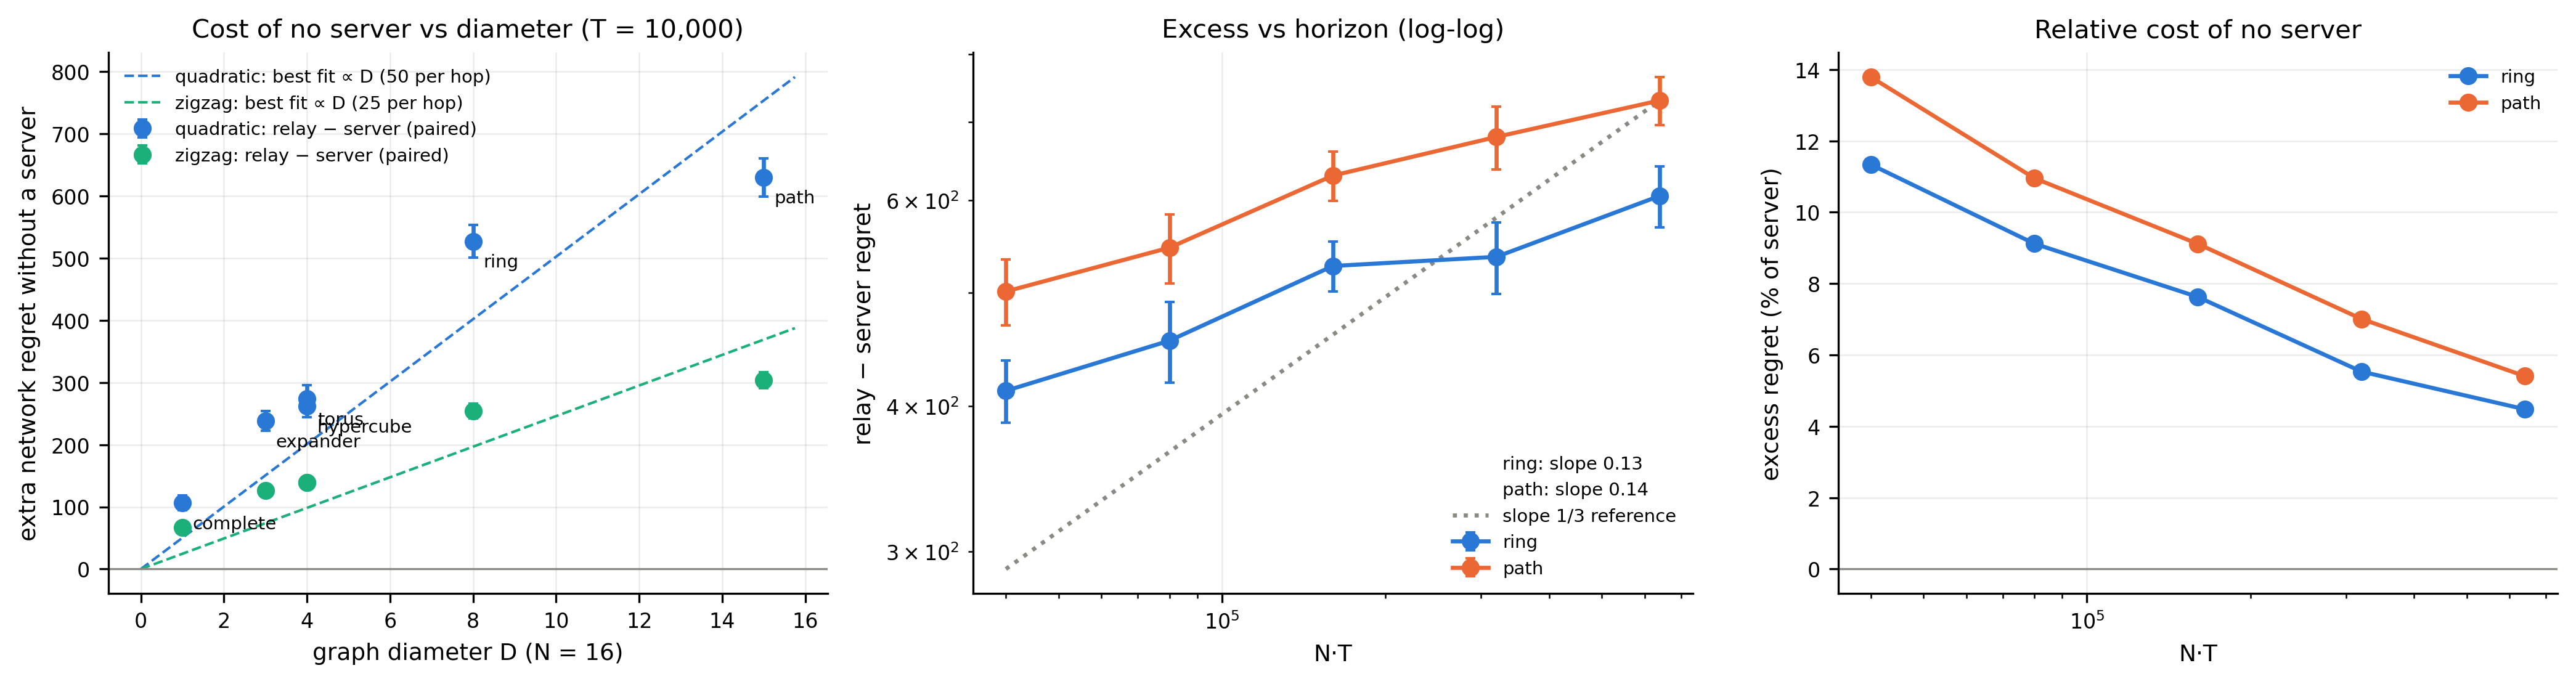
\includegraphics[width=\textwidth]{fig23_server_vs_serverless.png}
\caption{Theorem~\ref{thm:relay} against measurement (E23, $N=16$, 20 paired trials). Left: extra regret without a server grows sublinearly in the diameter $D$ (dashed: best fit $\propto D$). Middle: the excess is almost flat in $NT$ (slope 0.13--0.14 against the $1/3$ the bound predicts). Right: as a fraction of the server's regret it falls with the horizon.}
\label{fig:e23}
\end{figure}

\begin{figure}[H]
\centering
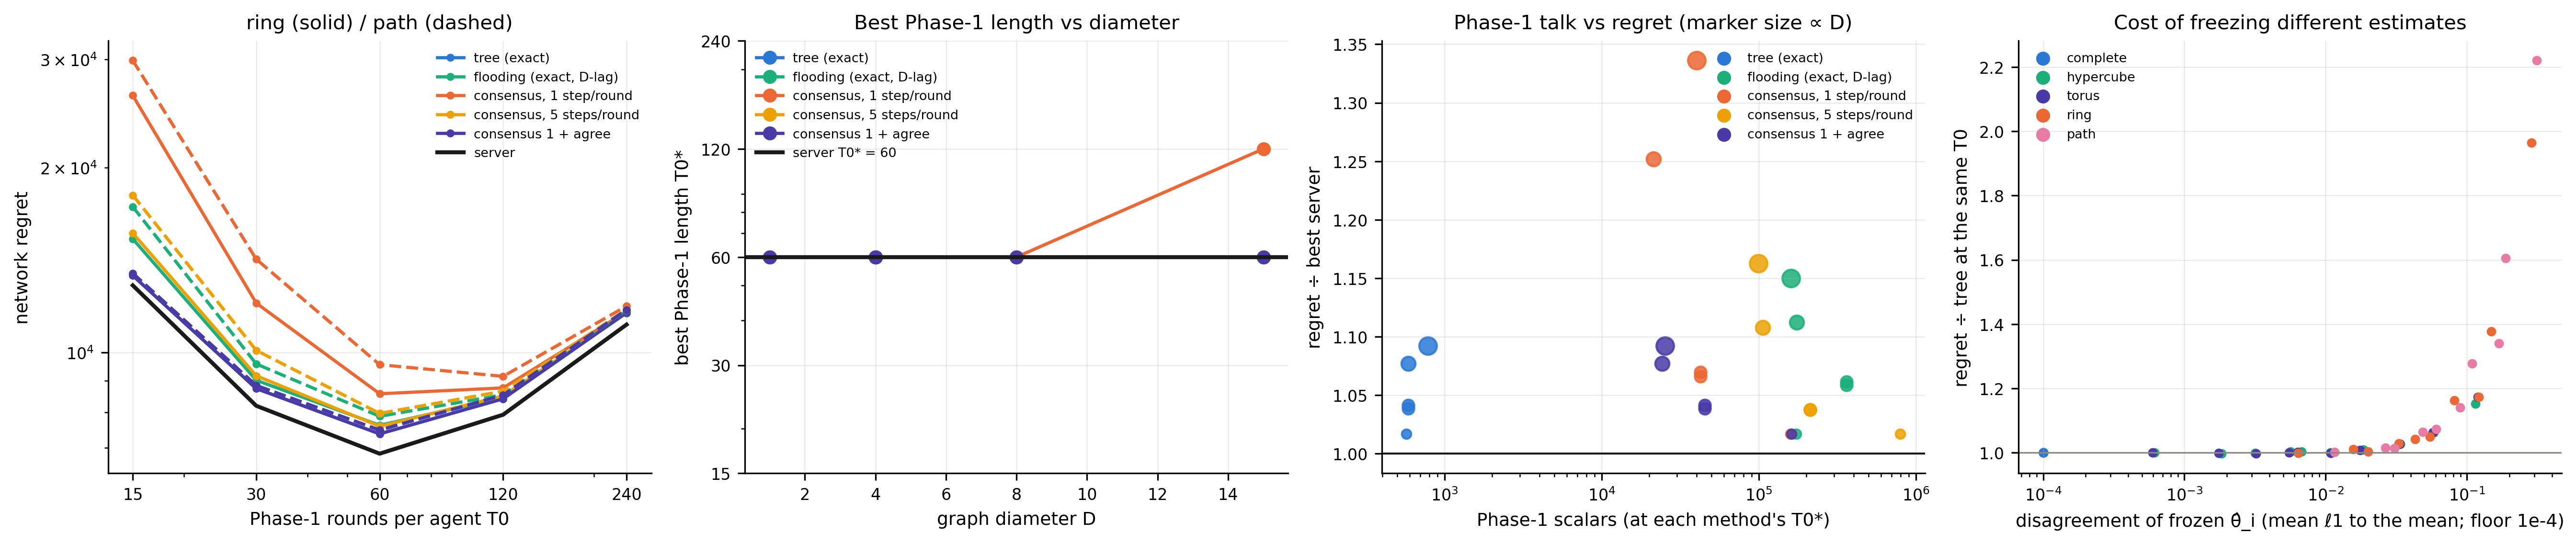
\includegraphics[width=\textwidth]{fig28_dec_coupling.png}
\caption{Exploration length and agreement on graphs (E28, $N=16$, 10 paired trials). From left: regret against the Phase-1 length $T_0$ on the ring and path; the best $T_0$ barely moves with $D$; Phase-1 communication against regret; and the regret cost of agents freezing different estimates, which one agreement pass at the freeze removes.}
\label{fig:e28}
\end{figure}

\begin{figure}[H]
\centering
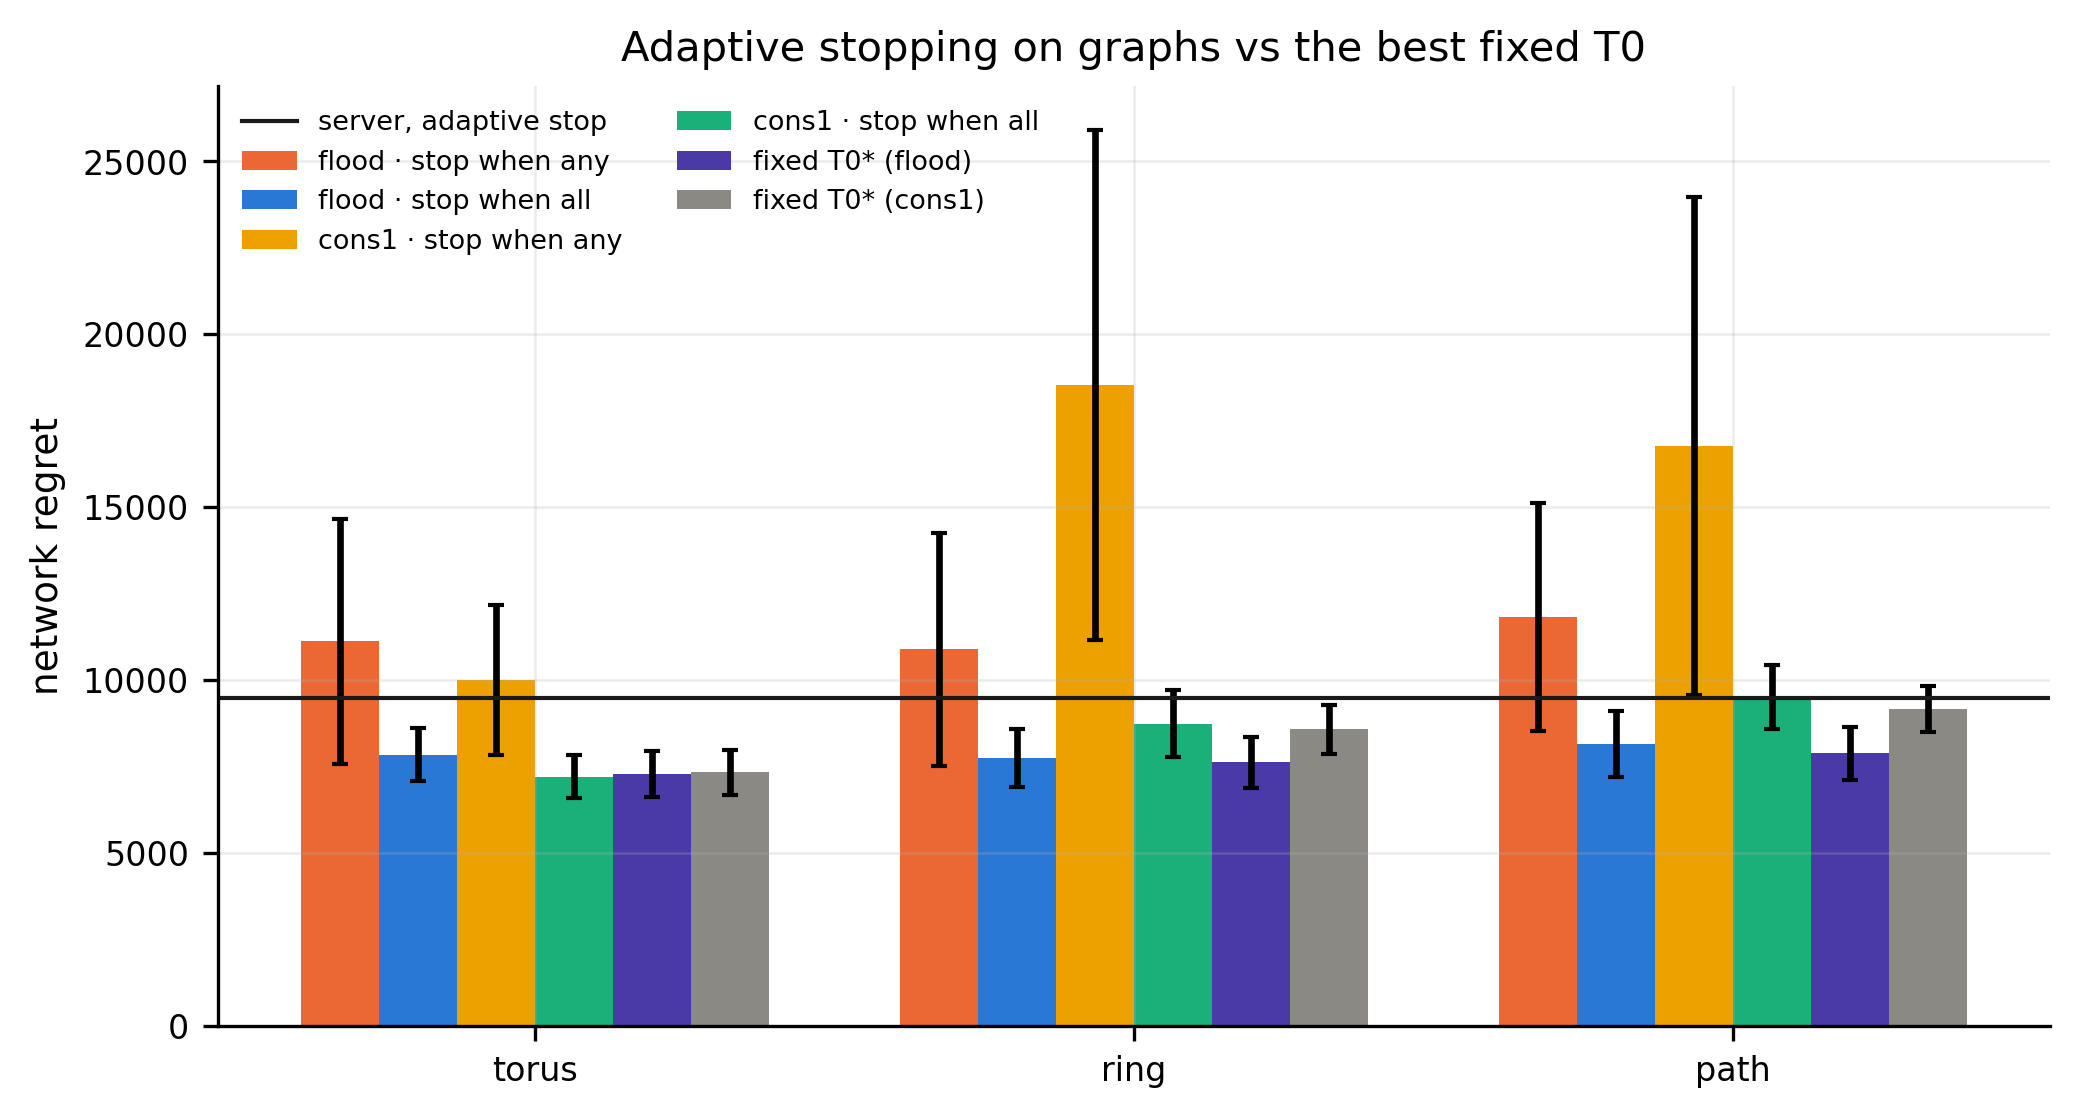
\includegraphics[width=0.6\textwidth]{fig28b_stop_rules.png}
\caption{Adaptive stopping on graphs (E28). ``Stop when any agent is stable'' costs 1.4--2.2$\times$ the regret of a fixed $T_0$; ``stop when all are'' is close to it but is modelled without its $\ge D$-round detection delay.}
\label{fig:e28b}
\end{figure}

\section{The regret--communication trade-off (notes and conjecture)}\label{sec:tradeoff}

Theorems~\ref{thm:upper} and~\ref{thm:comm} give \emph{one} point on the trade-off curve: optimal
regret with $O(\Nb\log NT)$ sync rounds. The natural question is the whole curve: with a budget of
$C$ sync rounds, what is the best achievable regret?

\paragraph{A heuristic lower bound.}
Between two syncs, agents share no information. Consider a sync-free window of length $L$ that
starts after the network has pooled $n$ samples. During it, the $N$ agents behave like $N$
learners with a common warm start, each learning only from its own $L$ pulls. In the single-agent
hard instance (Lemma~\ref{lem:dbglower}), the bins that must be distinguished have gaps of
order $(n+L)^{-1/3}$, and a lone learner needs $L^{2/3}$-type regret to resolve them. That
suggests
\[
R_T(N;C)\ \gtrsim\ \max\Big\{(NT)^{2/3},\ \max_{\text{windows}}N\,L^{2/3}\Big\},
\]
where the largest window is at least $T/C$ if syncs are spread evenly. Under this heuristic,
evenly spread syncs need $C\gtrsim\sqrt N$ to keep the second term below the first. Windows that
grow geometrically could need far fewer.

\begin{conjecture}
For single-index bandits with a server, the optimal regret $\tilde\Theta((NT)^{2/3})$ is
achievable with $\mathrm{polylog}(NT)$ sync rounds independent of $\Nb$. For batched Lipschitz
bandits, $O(\log\log T)$ batches suffice (Feng, Huang \& Wang 2022; to be checked), but that
algorithm eliminates arms it chooses to play. Here arms are given by contexts (sleeping bins),
which is exactly what our fixed-schedule experiments (E27, on branch \texttt{research/\allowbreak claims-evidence}) find breaks naive batching.
\end{conjecture}

\noindent What a paper would need: (a) a batch-aware Phase~2 (e.g.\ elimination over bins with
context-driven availability) with an upper bound in terms of $C$; (b) a matching lower bound that
formalises the window heuristic. Neither is done here.


\section*{Where the experiments are}
\begin{itemize}[nosep]
\item Theorem~\ref{thm:lower}/\ref{thm:upper} in practice: E22 (Figure~\ref{fig:e22}). One agent at
$NT$ against $N$ agents at $T$ with the same pooled exploration and bin width.
\item Theorem~\ref{thm:comm}: E22 part 2 (Figure~\ref{fig:e22b}), sync rounds and per-bin triggers
against $\log NT$.
\item Proposition~\ref{prop:share}: E24 (Figure~\ref{fig:e24}).
\item Theorem~\ref{thm:relay}: E23 and E28 (Figures~\ref{fig:e23}, \ref{fig:e28}, \ref{fig:e28b}).
\end{itemize}
\noindent The compression grid (E26) and the sync-schedule frontier behind
Section~\ref{sec:tradeoff} (E27) are on branch\\ \texttt{research/claims-evidence}.

\end{document}
